\section{Results}
\label{sec:result}
By comparing trips during the morning rush-hour (time window from
6am to 9am) to trips during the day until the start of
the evening rush-hour (9am to 5pm) one can easily see
how different user groups use the bike sharing program.

\begin{figure*}
\centering
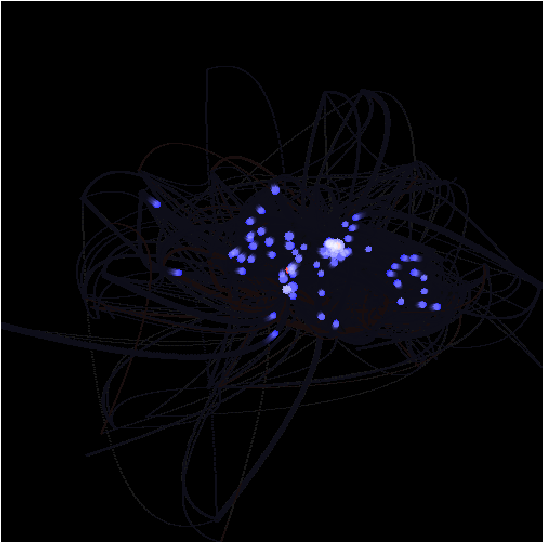
\includegraphics[width=3cm]{images/rush_7_tue.png}
\hspace*{0.5cm}
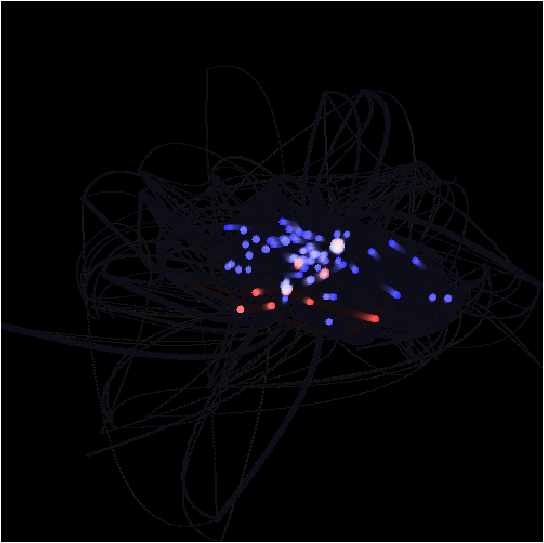
\includegraphics[width=3cm]{images/day_7_fri.png}
\hspace*{0.5cm}
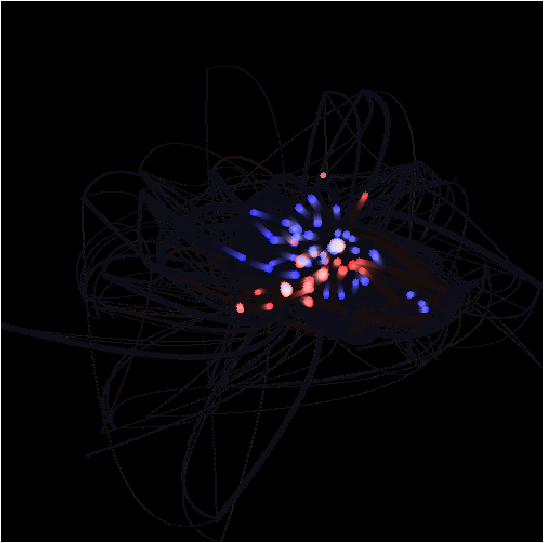
\includegraphics[width=3cm]{images/day_7_sun.png}
\hspace*{0.5cm}
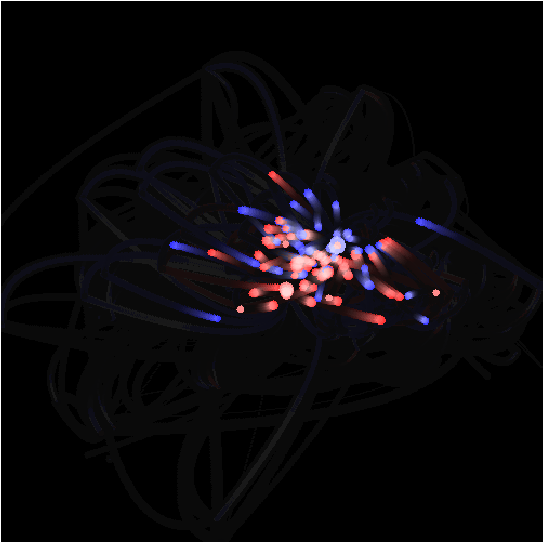
\includegraphics[width=3cm]{images/full_10_sun.png}
\hspace*{0.5cm}
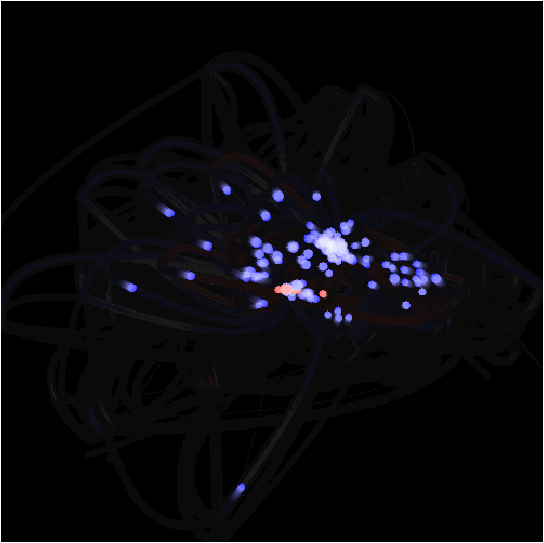
\includegraphics[width=3cm]{images/full_10_wed.png}
\caption{Different time slices. The leftmost image shows
bike usage during the morning rush hour, the second shows
bike usage during the day on a week day. The third image
shows bike usage during the day on a Sunday.
The last two images show the bike usage of two complete
days (relevant window is 24 hours), the first being a Sunday
and the second being a weekday. All images are during the summer months.}
\label{fig:smallm}
\end{figure*}
